%; whizzy paragraph -pdf xpdf -latex ./whizzypdfptex.sh
%; whizzy-paragraph "^\\\\begin{frame}"
% latex beamer presentation.
% platex, latex-beamer でコンパイルすることを想定。 

%     Tokyo Debian Meeting resources
%     Copyright (C) 2009 Junichi Uekawa
%     Copyright (C) 2009 Nobuhiro Iwamatsu

%     This program is free software; you can redistribute it and/or modify
%     it under the terms of the GNU General Public License as published by
%     the Free Software Foundation; either version 2 of the License, or
%     (at your option) any later version.

%     This program is distributed in the hope that it will be useful,
%     but WITHOUT ANY WARRANTY; without even the implied warreanty of
%     MERCHANTABILITY or FITNESS FOR A PARTICULAR PURPOSE.  See the
%     GNU General Public License for more details.

%     You should have received a copy of the GNU General Public License
%     along with this program; if not, write to the Free Software
%     Foundation, Inc., 51 Franklin St, Fifth Floor, Boston, MA  02110-1301 USA

\documentclass[cjk,dvipdfmx,12pt]{beamer}
\usetheme{Tokyo}
\usepackage{monthlypresentation}

%  preview (shell-command (concat "evince " (replace-regexp-in-string
%  "tex$" "pdf"(buffer-file-name)) "&")) 
%  presentation (shell-command (concat "xpdf -fullscreen " (replace-regexp-in-string "tex$" "pdf"(buffer-file-name)) "&"))
%  presentation (shell-command (concat "evince " (replace-regexp-in-string "tex$" "pdf"(buffer-file-name)) "&"))

%http://www.naney.org/diki/dk/hyperref.html
%日本語EUC系環境の時
\AtBeginDvi{\special{pdf:tounicode EUC-UCS2}}
%シフトJIS系環境の時
%\AtBeginDvi{\special{pdf:tounicode 90ms-RKSJ-UCS2}}

\title{第164回東京エリアDebian勉強会 \\ \\salsaと東京エリアdebian勉強会の\\Web/原稿システムの仕組み}
\subtitle{}
\author{Norimitsu Sugimoto (杉本 典充) \\dictoss@live.jp}
\date{2018-06-16}
\logo{
\includegraphics[width=8cm]{image200607/openlogo-light.eps}}

\begin{document}

\frame{\titlepage{}}

%\section{}

\begin{frame}{自己紹介}
  \begin{itemize}
  \item Norimitsu Sugimoto (杉本 典充)
  \item dictoss@live.jp
  \item Twitter: @dictoss
  \item Debian使って15年以上。sargeがtestingの頃から使っている
  \item 仕事はソフトウェア開発者をやってます
  \item pythonとDjangoの組み合わせで使うことが多いです
  \end{itemize}
\end{frame}

\begin{frame}{アジェンダ}
  \begin{itemize}
  \item はじめに
  \item 東京エリアDebian勉強会のシステム
  \item salsa.debian.org
  \item 東京エリアDebian勉強会のsalsaのシステム
  \item 今後の課題とまとめ
  \end{itemize}
\end{frame}

%\emtext{}

\begin{frame}[containsverbatim]{勉強会のシステム}
  \begin{itemize}
  \item webサイト
  \item 原稿データ、スライドデータのtexの原稿システム
  \item 参加者申し込み「connpass」
  \item DebianJPのメーリングリスト
  \end{itemize}
\end{frame}

\emtext{\url{salsa.debian.or}g}

\begin{frame}[containsverbatim]{salsaとは}
  \begin{itemize}
  \item \url{salsa.debian.org}
  \item Debianプロジェクトが2017年から運用を開始したプロジェクト管理サーバ
  \item gitlabが動作している
  \item Kubernetes(k8s)と連携したCI/CD処理
  \end{itemize}
\end{frame}

\begin{frame}[containsverbatim]{aliothからsalsaへの移行}
  \begin{itemize}
  \item 2003年からaliothというサーバが稼働し、FusionForgeが動作
  \item 2016年頃からFusionForgeの開発が滞る状況になる
  \item aliothの将来をどうするか議論が始まる
  \item Alioth Sprint 2017でsalsa誕生
  \item 2017年12月15日にsalsaのベータ運用が開始
  \item 2018年01月27日にsalsaの本運用が開始
  \item 2018年05月31日にalioth停止
  \end{itemize}
\end{frame}

\emtext{salsaの利用の仕方}

\begin{frame}[containsverbatim]{ドキュメント}
  \begin{itemize}
  \item \url{https://wiki.debian.org/Salsa/}
  \item \url{https://wiki.debian.org/Salsa/Doc}
  \item \url{https://docs.gitlab.com/}
  \end{itemize}
\end{frame}

\begin{frame}[containsverbatim]{アカウントの登録}
  \begin{itemize}
  \item Debian Developer
    \begin{itemize}
    \item debian.orgのメールアドレスでログイン可能
    \item LDAP連携している
    \end{itemize}
  \item Debian Developer以外
    \begin{itemize}
    \item \url{https://signup.salsa.debian.org/} でアカウントを作成する
    \item アカウントは、"-guest"という文字列が末尾につける必要あり
    \end{itemize}
  \end{itemize}
\end{frame}

\begin{frame}[containsverbatim]{チームの作成}
  \begin{itemize}
  \item gitリポジトリより前にまず「チーム」を作成する
  \item チームの作成は、\url{https://signup.salsa.debian.org/} で作成可能
  \item 作成したチームのページの例
    \begin{itemize}
      \item https://salsa.debian.org/tokyodebian-team
    \end{itemize}
  \item チームを作ったユーザは、初期設定でチームのOwner権限を割り当て
  \end{itemize}
\end{frame}

\begin{frame}[containsverbatim]{チームへのメンバの参加}
  \begin{itemize}
  \item チームをつくったあとは、協力してくれるメンバを増やしましょう
  \item \url{https://docs.gitlab.com/ee/user/permissions.html}
  \item チームのOwnerまたはMasterの権限を持っている人がユーザ追加できます
  \item メンバになりたい場合は「アクセス権限をリクエストする」ボタン押下で依頼できる
  \end{itemize}
\end{frame}

\begin{frame}[containsverbatim]{プロジェクトの作成}
  \begin{itemize}
  \item 画面上部からプロジェクトを追加できる
  \item 1つのプロジェクトにつき1つのgitリポジトリ
  \item 複数のgitリポジトリが欲しい場合は、チーム内に複数のプロジェクトを作る
  \end{itemize}
\end{frame}

\begin{frame}[containsverbatim]{CI/CD}
  \begin{itemize}
  \item CI(Continuous Integration)とCD(Continuous Delivery)
  \item git pushのタイミング、webhookなどでCI/CDを起動する
  \item gitlabはKubernetes(K8s)のインスタンスである"Runner"がCI/CD処理を実行する
  \item Shared Runners、Group Runners、Specific Runners
  \item Runnerサーバのスポンサーを募集中
  \end{itemize}
\end{frame}

\begin{frame}[containsverbatim]{ユーザ個人ページの設定}
  \begin{itemize}
  \item 「SSH Keys」ページからSSH鍵を登録できる
  \item git pull、git push時にSSH鍵で認証が済むため作業がスムーズ
  \end{itemize}
\end{frame}


\emtext{東京エリアDebian勉強会のsalsaのシステム}

\begin{frame}[containsverbatim]{aliothからsalsaへの移行の設計と作業内容}
  \begin{itemize}
  \item aliothが2018年5月31日で停止するため、salsaにデータを移行した
  \item gitリポジトリ、webサイト、PDFファイル配備の仕組みを移行した
  \item \url{https://wiki.debian.org/tokyodebian_salsa_migrate}
  \end{itemize}
\end{frame}

\begin{frame}[containsverbatim]{ファイルのライセンス}
  \begin{itemize}
  \item 東京エリアDebian勉強会のgitリポジトリに収録しているファイルのライセンスはGPLv2またはGPLv3
  \item 原稿やスライドデータを作成していただける方はライセンスをご了承の上、ご利用ください
  \end{itemize}
\end{frame}

\begin{frame}[containsverbatim]{チームとメンバ}
  \begin{itemize}
  \item Debian勉強会では「tokyodebian-team」というチーム名を利用
  \item メンバの権限ポリシーは定めていない
  \item コミット権をもらうにはメンバになる必要がある
  \item patchを投げる方法 \url{https://tokyodebian-team.pages.debian.net/prework-update.html}
  \end{itemize}
\end{frame}

\begin{frame}[containsverbatim]{静的ファイル公開機能:Pages}
  \begin{itemize}
  \item webサイトは \url{https://tokyodebian-team.pages.debian.net/} で公開中
  \item Pagesという静的ファイルのweb公開機能を使っている
  \item gitリポジトリ名をURLのホスト部の命名規則と同じにすると、"/"直下でファイル公開できる
  \item チーム内の他のプロジェクトは、 https://tokyodebian-team.pages.debian.net/pdf22018/ のようにプロジェクト名と同じディレクトリ名がつく
  \end{itemize}
\end{frame}

\emtext{webサイトの仕組み}

\begin{frame}[containsverbatim]{webサイトの仕組み}
  \begin{itemize}
  \item ソースコードは、\url{https://salsa.debian.org/tokyodebian-team/tokyodebian-team.pages.debian.net}
  \item Emacs Museを利用したhtmlテンプレートとデータからhtmlをビルドする仕組み
  \item git pushするとCI/CDを実行して、htmlを生成して自動配備する
  \item CI/CDの設定ファイルは、".gitlab-ci.yml"
  \item \url{https://tokyodebian-team.pages.debian.net/editing.html}
  \end{itemize}
\end{frame}

\begin{frame}[containsverbatim]{}
  \begin{figure}[H]
    \begin{center}
      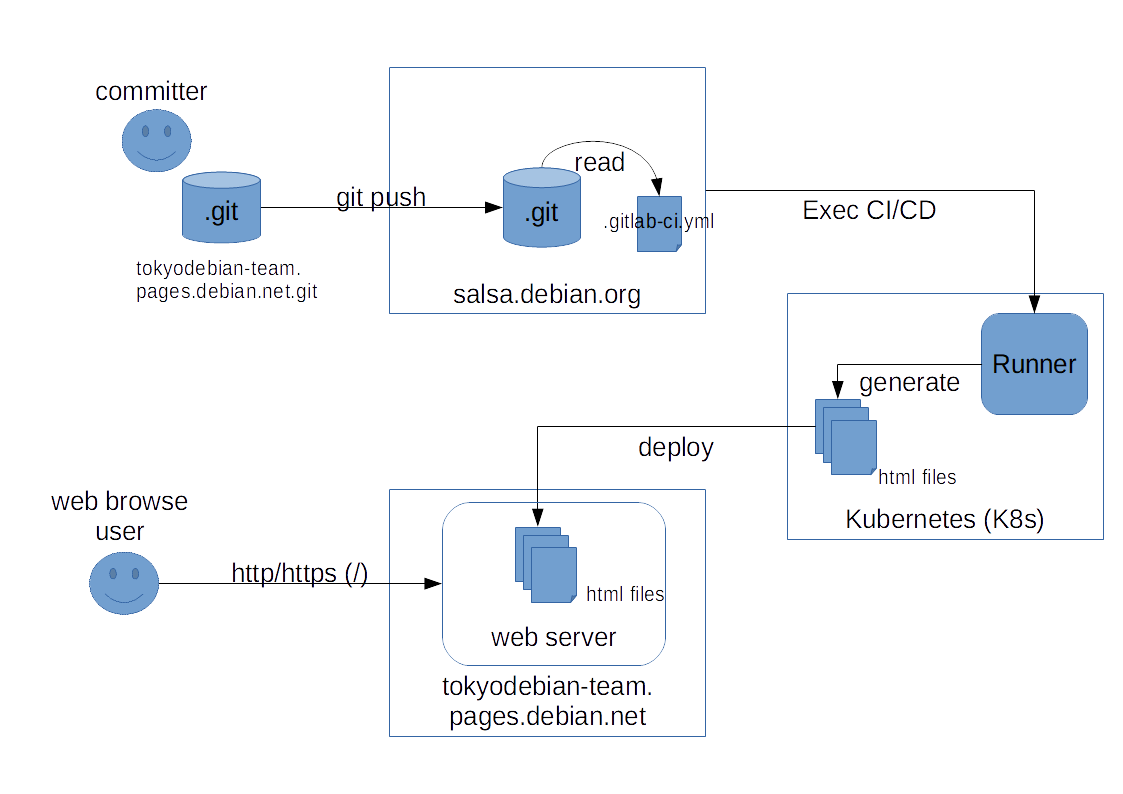
\includegraphics[width=10cm]{image201806/gitflow_web.png}
      \caption{webサイトへHTMLファイルを配備するCI/CD処理の流れ}
      \label{fig:deploy-html-CICD}
    \end{center}
  \end{figure}
\end{frame}


\emtext{原稿システムの仕組み}

\begin{frame}[containsverbatim]{原稿システムの仕組み}
  \begin{itemize}
  \item ソースコードは、\url{https://salsa.debian.org/tokyodebian-team/monthly-report}
  \item TeXを利用した組版システム。tex→dvi→pdfの順に変換して原稿ファイルになる
  \item 有志によって原稿とスライドのテンプレートを作成
  \item 豊富な原稿量は勉強会参加者の長年の積み重ね
  \end{itemize}
\end{frame}

\begin{frame}[containsverbatim]{原稿システムの複数gitの使い分け}
  \begin{itemize}
  \item texのgitリポジトリと、公開用pdfファイルのgitリポジトリは分けている
  \item "pdf2005.git"から"pdf2018.git"に分割し、gitリポジトリの中にビルドしたpdfファイルをコミットしている
  \item CI/CDはtexのgitリポジトリでは行っていない
  \item CI/CDは"pdf20yy.git"のgitリポジトリへのpush時に処理し、"/pdf20yy/xxx.pdf"のパスでweb公開している
  \end{itemize}
\end{frame}

\begin{frame}[containsverbatim]{PDFファイルを配備するCI/CD処理の流れ}
  \begin{figure}[H]
    \begin{center}
      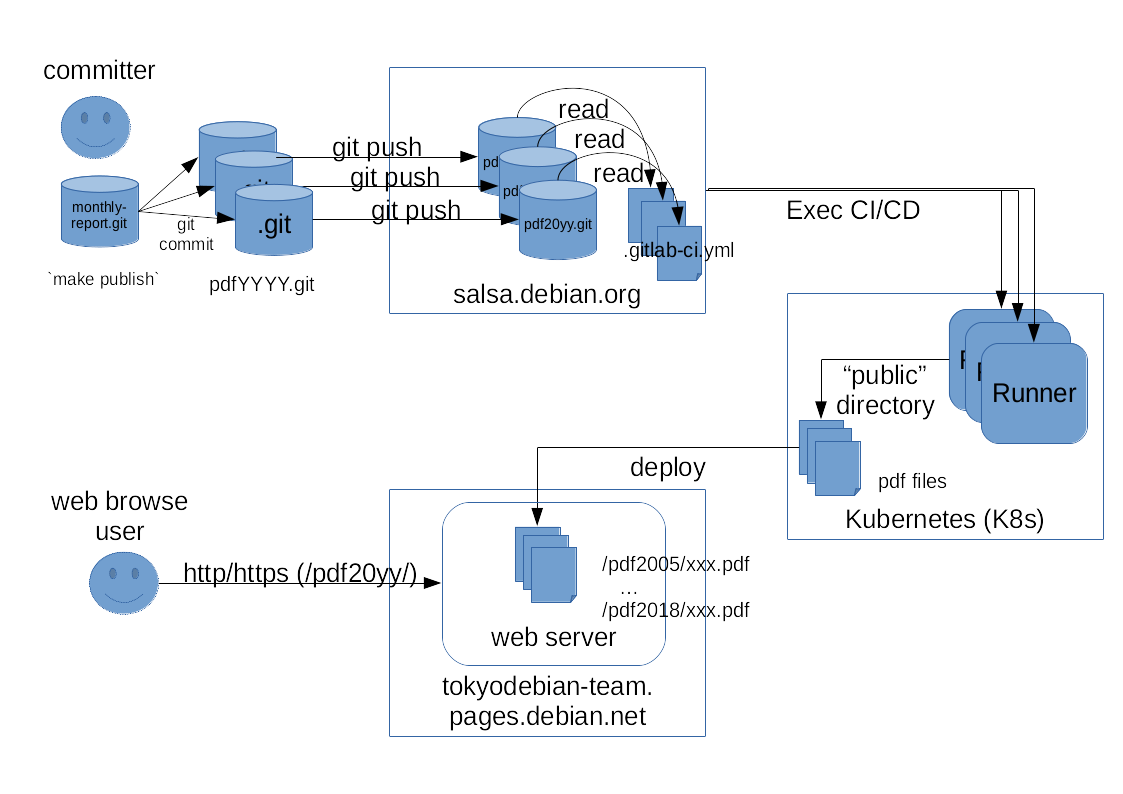
\includegraphics[width=10cm]{image201806/gitflow_pdf.png}
      \caption{webサイトへ原稿及びスライドPDFファイルを配備するCI/CD処理の流れ}
      \label{fig:deploy-pdf-CICD}
    \end{center}
  \end{figure}
\end{frame}

\begin{frame}[containsverbatim]{今後の課題}
  \begin{itemize}
  \item 原稿システムのCI/CD処理に失敗することがある
  \item webサイトをリニューアルしたい
  \item 原稿ファイルとtexビルドシステムのUTF-8対応
  \item 原稿の寄贈が減ってきており、半年のまとめ冊子のページ数が減ってきている
  \end{itemize}
\end{frame}


\begin{frame}[containsverbatim]{まとめ}
  \begin{itemize}
  \item salsaで提供しているgitlabの機能と設定を紹介しました
  \item 東京エリアDebian勉強会のwebサイト、原稿システムをsalsaへ移行しました
  \item 資料の作成と公開は、自分の学びになるだけでなく、他の参加者の学びにもなると思います
  \end{itemize}
\end{frame}


%\begin{frame}{参考文献}
%  \begin{itemize}
%  \item a
%  \end{itemize}
%\end{frame}

\end{document}


;;; Local Variables: ***
;;; outline-regexp: "\\([ 	]*\\\\\\(documentstyle\\|documentclass\\|emtext\\|section\\|begin{frame}\\)\\*?[ 	]*[[{]\\|[]+\\)" ***
;;; End: ***
